%
% PROJECT: <ETD> Electronic Thesis and Dissertation Initiative
%   TITLE: LaTeX report template for ETDs in LaTeX
%  AUTHOR: Neill Kipp, nkipp@vt.edu
%     URL: http://etd.vt.edu/latex/
% SAVE AS: etd.tex
% REVISED: September 6, 1997 [GMc 8/30/10]
% 

% Instructions: Remove the data from this document and replace it with your own,
% keeping the style and formatting information intact.  More instructions
% appear on the Web site listed above.

\documentclass[12pt]{report}

\setlength{\textwidth}{6.5in}
\setlength{\textheight}{8.5in}
\setlength{\evensidemargin}{0in}
\setlength{\oddsidemargin}{0in}
\setlength{\topmargin}{0in}

\setlength{\parindent}{0pt}
\setlength{\parskip}{0.1in}

% Uncomment for double-spaced document.
% \renewcommand{\baselinestretch}{2}
\usepackage{graphicx}
\usepackage{epstopdf}
\usepackage{listings}
\usepackage{color}
\usepackage{subfig}
\usepackage{floatrow}
\usepackage{tikz}
\usepackage{hyperref}
\hypersetup{
    colorlinks,
    citecolor=black,
    filecolor=black,
    linkcolor=black,
    urlcolor=black
}
% \usepackage{epsf}

\begin{document}

\thispagestyle{empty}
\pagenumbering{roman}
\begin{center}

% TITLE
{\Large 
Replication of Concurrent Applications in a Shared Memory Multikernel
}

\vfill

Yuzhong Wen

\vfill

Thesis submitted to the Faculty of the \\
Virginia Polytechnic Institute and State University \\
in partial fulfillment of the requirements for the degree of

\vfill

Master of Science \\
in \\
Computer Science and Application

\vfill

Binoy Ravindran, Chair \\
Ali R. Butt Co-Chair \\
Dongyoon Lee

\vfill

June 17, 2016 \\
Blacksburg, Virginia

\vfill

Keywords: blah, blah
\\
Copyright 2016, Yuzhong Wen

\end{center}

\pagebreak

\thispagestyle{empty}
\begin{center}

{\large Replication of Concurrent Applications in a Shared Memory Multikernel}

\vfill

Yuzhong Wen

\vfill

(ABSTRACT)

\vfill

\end{center}

Lorem ipsum dolor sit amet, consectetur adipiscing elit. Nunc nec elit molestie, mattis mi a, consequat arcu. Fusce venenatis rhoncus elit. Morbi ornare, libero a bibendum pretium, nibh orci tristique mauris, in suscipit mauris nibh ac metus. Nullam in sem vitae nisi aliquet iaculis in a nibh. Aliquam lobortis quis turpis ut tempus. Sed eu sapien eu nisi placerat viverra pharetra eu turpis. Mauris placerat massa mi, auctor facilisis sem consequat in. Pellentesque sollicitudin placerat mi quis rhoncus. In euismod lorem semper, scelerisque leo et, dapibus diam. Suspendisse augue dui, placerat at finibus a, cursus vitae erat. Nam accumsan magna vitae lorem tincidunt, et rhoncus elit consequat.

Suspendisse ut tellus at ex suscipit sollicitudin ut ut elit. Nam malesuada molestie elit eget luctus. Donec id quam ullamcorper, aliquam mauris at, congue felis. Nunc dapibus dui sit amet nisl laoreet, eget rhoncus est tempor. Mauris in blandit mauris. Aenean vitae ipsum lacinia, blandit turpis et, feugiat purus. Mauris in finibus quam, ac dictum lorem. Nam dignissim luctus ante. Suspendisse risus felis, imperdiet a lobortis sed, suscipit ac dui. Nullam fermentum velit eu congue dictum. Pellentesque tempor dui vel nisl tristique, non sollicitudin odio elementum. In ultricies elementum mattis.

Vestibulum eget imperdiet eros. Proin bibendum sit amet felis quis dignissim. Aliquam convallis mauris ut sapien gravida, eu consequat lacus dignissim. Vivamus porttitor hendrerit nisl, sit amet suscipit lorem vestibulum ut. Donec id tellus condimentum, sollicitudin sapien vel, lobortis nulla. Donec et elit quis est tempor semper. Aliquam erat volutpat. In nec consectetur dui. Nullam aliquam diam at eros ultrices vehicula. Nulla nibh ex, condimentum vitae nisl sed, aliquet ultricies sapien. Suspendisse potenti. Suspendisse pellentesque tincidunt facilisis. Morbi sodales vulputate ex malesuada molestie. Vestibulum eget placerat nunc.
\vfill

% GRANT INFORMATION

This work is supported by AFOSR under the grant FA9550-14-1-0163.  Any opinions, findings, and conclusions expressed in this thesis are those of the author and do not necessarily reflect the views of AFOSR.

\pagebreak

% Dedication and Acknowledgments are both optional
% \chapter*{Dedication}
% \chapter*{Acknowledgments}

\tableofcontents
\pagebreak

\listoffigures
\pagebreak

\listoftables
\pagebreak

\pagenumbering{arabic}
\pagestyle{myheadings}

\newcommand{\detstart}{\_\_det\_start}
\newcommand{\detend}{\_\_det\_end}
\newcommand{\dettick}{\_\_det\_tick}

\chapter{Introduction}
% 1. single machine replication
% 2. state machine replication
% 2.1 weak determinism, total order of synchronization primitives.
% 3. contribution
% 3.1 deterministic execution and schedule replication inside kernel
% 3.2 fully transparent, minimal modification to application
% 3.3 comparision that sched rep is better

% cite a bunch of intra-machine solutions
% Hypervisor-based Fault-tolerance
% Operating System Support for Redundant Multithreading
% Tardigrade: Leveraging Lightweight Virtual Machines to Easily and Efficiently Construct Fault-Tolerant Services

State machine replication (SMR) has been widely used for fault-tolerance purpose in nowadays computing services. In SMR, it models the service to be replicated with a set of inputs, a set of outputs and a set of states. The replication system ensures that for a given input set, from the same initial state, the replicas can produces the same state transition which in turn leads to the same result. Such a system is able to be resilient to failures in one or more replicas (depends on how many replicas are there in the system). To provide such property, determinism is required for the state machine, otherwise state machines will get diverged in different states even with the same input set.

% A section for server applications
% Practical and Low-Overhead Masking of Failures of TCP-Based Servers

\section{Contributions}

This thesis addresses the following contributions:

\begin{itemize}
\item Based on Popcorn Linux, we implemented two different replication modes in the kernel, Deterministic Execution and Schedule Replication. to synchronize thread inter-leavings of replicated concurrent applications. They achieved the same goal in two different directions: Deterministic Execution uses a deterministic algorithm to decide the order of execution on both primary and secondary; while Schedule Replication enforces the secondary replica to follow the non-deterministic execution order that happened previously on the primary kernel.

\item Two different replication modes share the same programming interface. By wrapping a code section with \detstart\ and \detend\ system calls, the execution order of wrapped sections can be the same on both primary and secondary kernel. Based on this common interface, we also provide a set of runtime supports that allows the user to run applications on our system with minimal code modification.

\item To explore the pros and cons for both replication modes, we evaluated different types of concurrent applications on our system. For computational application we had maximum 63.39\% slowdown for Deterministic Execution and maximum 36.3\% slowdown for Schedule Replication. For two web servers we had maximum 25.22\% slowdown for Deterministic Execution and maximum 1.96\% slowdown for Schedule Replication. Both replication modes achieved decent overhead for production use, but Schedule Replication is the better replication mode for most of our use case, in terms of both simplicity and lower overall overhead.
\end{itemize}
\chapter{Popcorn Linux Background}
\chapter{Deterministic Execution}
Deterministic execution provides a property that given the same input, a multithreaded program can always generate the same output. Such a system fits perfectly for our replication purpose. As long as the primary and secondary receive the same input, the replicated application will sure end up with the same state and generate the same output.

For multi-threaded programs, an observation is that as long as the threads don't communicate with each other, the execution is sure to be deterministic\cite{devietti2009dmp}. For example, in pthread based programs, all the inter-thread communications are synchronized by pthread primitives. By making the interleaving of sychronization primitives to be deterministic, the entire program is sure to be deterministic. With this observation, some runtime deterministic solutions actually enforce determinism by trapping pthread primitives\cite{cui2013parrot}\cite{liu2011dthreads}\cite{olszewski2009kendo}. This type of deterministic system is called "Weak Deterministic System". It assumes that the applications are data race free, and only guarantee the deterministic interleaving of thread synchronization primitives such as mutex locks and condition variables. Our implementation falls into this category, but unlike other runtime deterministic systems, our runtime does not directly trap pthread primitives, but provides two system calls for programmer to define a deterministic section. The runtime maintains a global execution order, according to this order, an execution token is passed among all the tasks deterministically. Only the task with the execution token can enter the deterministic area, and the token will be held on this task only if it leaves its deterministic area.

This chapter is structured as follows:
\begin{itemize}
\item Section \ref{sec:detsched} shows the basic algorithm and programming interface of the deterministic system.
\item Section \ref{sec:logimbalance} explains the logical time imbalance problem of this algorithm and two solutions for two different cases.
\item Section \ref{sec:edeadlock} shows the case which might cause deadlock, and the solution to it.
\end{itemize}

\section{Logical Time Based Deterministic Scheduling} \label{sec:detsched}
Inspired by Kendo and Conversion, this scheduling policy maintains a logical time for each task inside the current Popcorn namespace. Our system provides three system calls for the applications to control the thread-interleaving:
\begin{itemize}
   \item \_\_det\_start: When it is called, only the task holds the minimal logical time can proceed, if several tasks have the same logical time, the one who has the smallest PID number gets the turn. If the current thread is able to proceed, this thread will be marked as "in a deterministic section".
   \item \_\_det\_end: When it is called, the system will increase the current thread's logical time by 1, and marks it as "out of a deterministic section".
   \item \_\_det\_tick: This system call comes with a parameter of an integer. When it is called, the logical time will be increased by value defined by the parameter.
\end{itemize}.

\begin{figure}
\centering
\begin{lstlisting}[numbers=left, frame=single, basicstyle=\small, breaklines]{blah}
void producer() {
    while (running){
        item = generate_item();
	    syscall(__NR_det_start);
	    pthread_mutex_lock(mutex);
	    syscall(__NR_det_end);    
	    putItem(queue, item);    
	    pthread_mutex_unlock(mutex);
    }
}

void consumer() {
    while (running){
        syscall(__NR_det_start);
        pthread_mutex_lock(mutex);
        syscall(__NR_det_end);
        item = getItem(queue);    
        pthread_mutex_unlock(mutex);		
        consume_item(item);
    }
}
\end{lstlisting}
\caption{An example use of the deterministic syscalls}
\label{fig:example}
\end{figure}
Figure~\ref{fig:example} shows an example use of the system calls. Simply wrap pthread\_mutex\_lock with \_\_det\_start and \_\_det\_end will make the acquisition of the mutex to be deterministic.

If the logical time is updated but the one has the minimal logical time is sleeping in \_\_det\_start, the one whose updates the tick will wake the sleeping one up. As long as the replicated application updates logical time in a same way on both primary and secondary, they will sure end up with the same thread interleaving. Figure~\ref{f:algorithm} shows a simplified version of this algorithm (some mutual exclusion points are omitted here).

To make an application to run in a deterministic way, one should put \_\_det\_start and \_\_det\_end around the synchronization primitives such as pthread\_mutex\_lock and pthread\_spin\_lock, so that the order of getting into critical sections is controlled under our deterministic scheduling.

\begin{figure}
\begin{lstlisting}[numbers=left, frame=single, basicstyle=\small, breaklines]{blah}
void __det_start()
{
    if (token->token != current)
        sleep(current);
    current->ft_det_state = FT_DET_ACTIVE;        
}
void __det_end()
{
    current->ft_det_state = FT_DET_INACTIVE;
    __update_tick(1);
}
void __det_tick(int tick)
{
    __update_tick(tick);
}
void __update_tick(int tick)
{
    current->tick += tick;
    token = find_task_with_min_tick(ns);
    if (is_waiting_for_toUponken(token->task))
    	wake_up(token->task);
}
\end{lstlisting}
\caption{Simplified implementation of deterministic system calls}
\label{f:algorithm}
\end{figure}

\section{Balance the Logical Time} \label{sec:logimbalance}
Only increasing the logical time by 1 at \detend\ isn't enough. With an example we show how this could break the scalability and how to mitigate this problem. In Figure~\ref{fig:imbalance}, we show a particular execution point of the producer-consumer model in the program snippet we presented in Figure~\ref{fig:example}, solid lines represents the path that is already executed. In this case, consumer reaches consumeItem with logical time 3 and has the token. Assume the real execution time of consumeItem is 10s, which means that when the consumer reaches \_\_det\_end, it would be at least 10s later, that is, the producer has to wait at \_\_det\_start for at least 10s. However we've already enforces the access order of the mutex, the execution out of the critical section should go in parallel since threads don't communicate at that point, in worst case, this kind of waiting will turn a parallel program into a serial program.

\begin{figure}
\centering
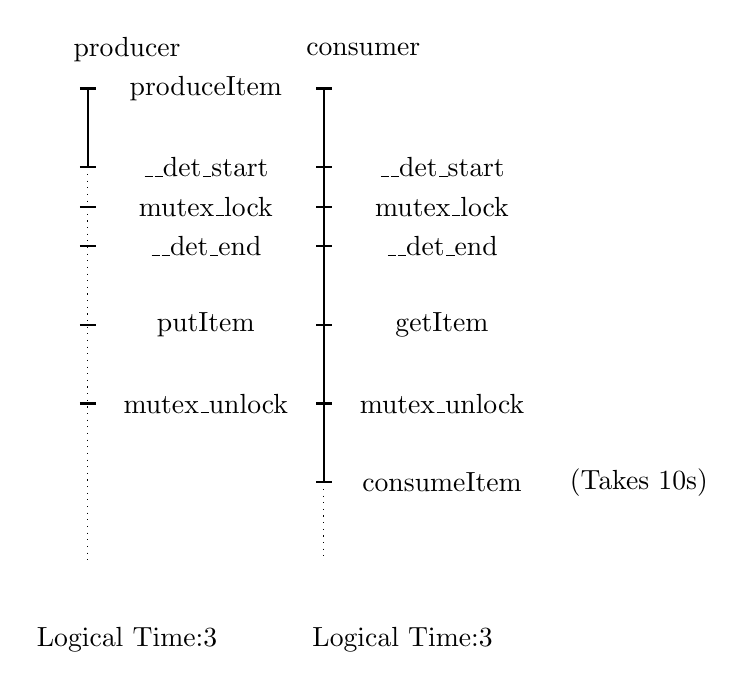
\begin{tikzpicture}
   \draw[thick] (0,4) --  (0,5); 
   \draw[dotted] (0,4) --  (0,-1);
   
   \node[align=right] at (0.5,5.5) {producer};
   \node[align=right] at (1.5,5) {produceItem};
   \draw[thick] (-0.1,5) -- (0.1,5);
   \node[align=right] at (1.5,4) {\_\_det\_start};
   \draw[thick] (-0.1,4) -- (0.1,4);
   \node[align=right] at (1.5,3.5) {mutex\_lock};
   \draw[thick] (-0.1,3.5) -- (0.1,3.5);
   \node[align=right] at (1.5,3) {\_\_det\_end};
   \draw[thick] (-0.1,3) -- (0.1,3);
   \node[align=right] at (1.5,2) {putItem};
   \draw[thick] (-0.1,2) -- (0.1,2);
   \node[align=right] at (1.5,1) {mutex\_unlock};
   \draw[thick] (-0.1,1) -- (0.1,1);   
   \node[align=right] at (0.5,-2) {Logical Time:3};
   
   \draw[thick] (3,0) --  (3,5); 
   \draw[dotted] (3,0) --  (3,-1);
   
   \node[align=right] at (3.5,5.5) {consumer};
   \node[align=right] at (4,5) {};
   \draw[thick] (2.9,5) -- (3.1,5);
   \node[align=right] at (4.5,4) {\_\_det\_start};
   \draw[thick] (2.9,4) -- (3.1,4);
   \node[align=right] at (4.5,3.5) {mutex\_lock};
   \draw[thick] (2.9,3.5) -- (3.1,3.5);
   \node[align=right] at (4.5,3) {\_\_det\_end};
   \draw[thick] (2.9,3) -- (3.1,3);
   \node[align=right] at (4.5,2) {getItem};
   \draw[thick] (2.9,2) -- (3.1,2);
   \node[align=right] at (4.5,1) {mutex\_unlock};
   \draw[thick] (2.9,1) -- (3.1,1);
   \node[align=right] at (4.5,0) {consumeItem};   \node[align=right] at (7,0) {(Takes 10s)};
   \draw[thick] (2.9,0) -- (3.1,0);
   \node[align=right] at (4,-2) {Logical Time:3};   
\end{tikzpicture}
\caption{An example of logical time imbalance.}
\label{fig:imbalance}
\end{figure}

Generally, logical time imbalance can happen in two cases:
\begin{itemize}
  \item A task is running for a long time (in user space).
  \item A task is sleeping for a long time (in kernel space).
\end{itemize}

In the upcoming sections we will discuss the solution of each of the cases.
\subsection{Execution Time Profiling}
When a task is running in a computational region (in user space) which might take a long time, the logical time of the task should increase along with the execution. In Kendo this is done by counting retired read instructions — using performance counters — to track to progress of a running task and increases its logical time accordingly. However it is hard to ensure that on the primary and the secondary the performance counter can have the same behaviour, as a result we have to find another way to track the progress of a running task.

Instead of deciding the logical time during the runtime, we discovered a way to settle the logical time during the compilation time. The basic idea is to collect the execution time of via a profile run, then compile the application with the data from the profile run. Based on LLVM, we implemented two compiler passes to do the profiling and instrumentation.

\paragraph{Profile Pass}
In order to get the execution time of a program, we make a profile pass to collect the execution time at the granularity of basic block. During the compilation time, this compiler pass will assign a unique number to each basic block, and inserts time profiling functions around every basic block beyond a certain threshold in terms of number of instructions. The profile run is launched by our profile launcher, which will keep track of the execution time of the application, and compute the average execution time for each instrumented basic block upon the application exits. In the end, all the gathered information will be output to a file for future use.

\paragraph{Logical Time Pass}
After the program finished one profile run with the instrumentation of profile pass, we can launch our compiler again to generate the final executable. The logical time pass will take the profile data file as input. This time at the end of each basic block, a \_\_det\_tick will be inserted with the parameter of a scaled execution time of the current basic block. So that the logical time will be bumped at the end of each basic block according to the actual execution time of each basic block. Fiin gure~\ref{fig:instrumented} shows an example of instrument basic block in LLVM-IR. In this example, Line 9 is the end of the basic block, it comes with a \dettick\ system call with a value 2895535, which is generated and normalized from a previous profile run. In this basic block, line 5 is the most time consuming part in the entire program (pbzip2), as a result this basic block needs a relatively large tick increment.

\begin{figure}
\centering
\begin{lstlisting}[numbers=left, frame=single, basicstyle=\small, breaklines]
  %bufSize24 = getelementptr inbounds %struct.outBuff, %struct.outBuff* %35, i32 0, i32 1
  %36 = load i32, i32* %bufSize24, align 4
  %37 = load i32, i32* @_ZL12BWTblockSize, align 4
  %38 = load i32, i32* @_ZL9Verbosity, align 4
  %call25 = call i32 @BZ2_bzBuffToBuffCompress(i8* %32, i32* %outSize, i8* %34, i32 %36, i32 %37, i32 %38, i32 30)
  store i32 %call25, i32* %ret, align 4
  %39 = load i32, i32* %ret, align 4
  %cmp26 = icmp ne i32 %39, 0
  %40 = call i32 (...) @syscall(i32 321, i64 2895535)
  br i1 %cmp26, label %if.then.27, label %if.end.29

\end{lstlisting}
\caption{An instrumented basic block in pbzip2 with dettick.}
\label{fig:instrumented}
\end{figure}

\newpage

%Compiler shit here

\subsection{Tick Bumping for External Events}

When a task is sleeping in the kernel, usually it is in a system call and waiting for some events to wake it up. Especially for system calls like epoll\_wait, poll and accept and other I/O system calls, the arrival time of the event is non-deterministic, as a result, we cannot simply use \dettick\ to increase the logical time with a predefined value from a profile run, because we have no idea how long the thread will be sleeping in the kernel.

Some deterministic systems simply remove the sleeping tasks out of the deterministic schedule and put them back after they are back to user space. This is not applicable in a replication system like ours, as previously stated, the wake up time of those system calls might be different from the primary and secondary replica. As a result we must not abandon those sleeping tasks, and have to maintain the consistent state of the logical time for those tasks.

\begin{figure}
\centering
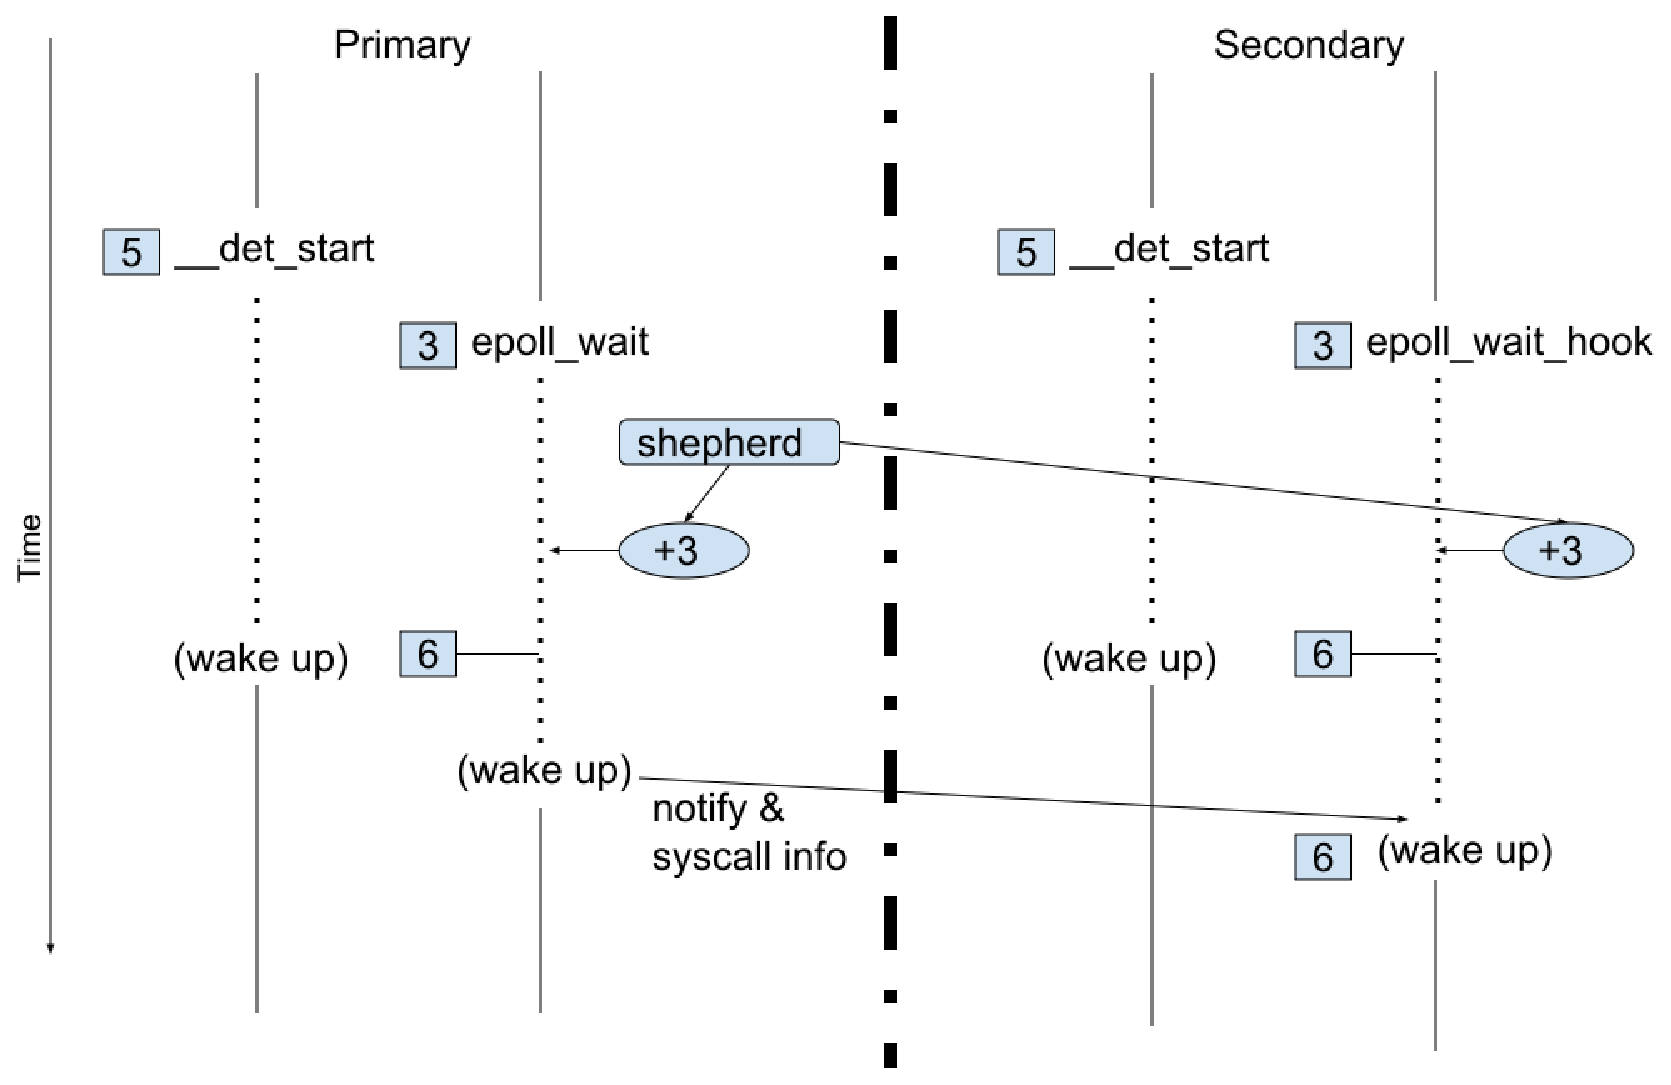
\includegraphics[width=0.8\columnwidth]{figures/tickbump}
\caption{An example of tick bumping}
\label{f:tick_bump}
\end{figure}

In order to let the token passing keep going with those blocking system calls, we need a way to keep bumping those thread's logical time while they are sleeping, a "Tick Shepherd" is implemented to dynamically bump the logical time of the threads that are sleeping in such system calls. The Tick Shepherd is a kernel thread which is mostly sleeping in the background, whenever the token is passed on to a thread that is sleeping on external events or a thread is going to sleep with the token, the shepherd will be woken up to increase the sleeping thread's logical time and send the increased value to the replica. In the meanwhile the corresponding system call on the replica will be blocked at the entry point, and bumps its logical time according to the information from the primary. The syscall on the secondary doesn't proceed until the primary returns from the syscall. In this way we can make sure that when both of the syscalls wake up from sleeping, all the replicas will end up with a consistent state, in terms of logical time. The Tick Shepherd will keep bumping sleeping tasks logical time until for a given period the state of all the tasks comes to a stable point, where nobody makes a single syscall. After that, it will go back to sleep again.


Figure~\ref{f:tick_bump} shows an example of how Tick Shepherd works in action. In this example, tick shepherd detects the token is on a thread sleeping in epoll\_wait, so it bumps its tick by 3 and sends this info to the secondary so that the token can leave this thread. And after the primary returns from epoll\_wait, it sends a message to the secondary, so that the corresponding thread can start to execute its epoll\_wait and uses the output from the primary as its own output.


We only let Tick Shepherd to bump the system calls that for sure will be called for deterministic times, the current implementation covers all the major I/O related system calls.

\section{Eliminate Deadlocks} \label{sec:edeadlock}
% cite futex and glic here
With wrapping all the pthread\_mutex\_lock with our deterministic system calls, there is a potential risk of having deadlocks. Serializing all the lock acquisitions with our implementation basically means putting a giant global mutex lock around every lock acquisition. As shown in Figure~\ref{fig:deadlock}, Thread 2 has a lower logical time and try to acquire the mutex(b), however mutex(b) is contended, as a result Thread 2 will call futex\_wait and put the thread into sleep until mutex(b) is released by someone else. At this point, Thread 2 will never increase its logical time until mutex(b) is released. So Thread 1 will never goes through the \_\_det\_start, and it will never unlock mutex(b), which means Thread 2 will never be woken up.

Since we already know that a contented mutex will call futex\_wait to wait for a unlock event, the solution to this deadlock problem is to temporary remove the thread in futex\_wait out of the deterministic schedule, and add it back when it returns from futex\_wait. In the example of Figure~\ref{fig:deadlock}, Thread 1 will be able to proceed its \_\_det\_start and keep executing. In order to not to break the determinism, we guarantee the following:
\begin{itemize}
\item We guarantee that the waiting queue in futex\_wait is strictly FIFO, which means the wakeup sequence will be the same as the sequence of getting into futex\_wait. Since the latter one is ensured by our \_\_det\_start, with this hack to futex, the wake up sequence from futex\_wait will be the same sequence determined by previous \_\_det\_start. This is implemented by fixing the priority of each futex object, so that the priority queue inside futex\_wait can behave like a FIFO queue.
\item We guarantee that when waking up from a futex\_wait, the thread always waits for the token before returning to the user space. With this implemented, the timing (in terms of logical time) of getting out of a contended pthread\_mutex\_lock will be deterministic. This is implemented by adding a \_\_det\_start after the wake up point of futex\_wait.
\end{itemize}

\begin{figure}
\centering
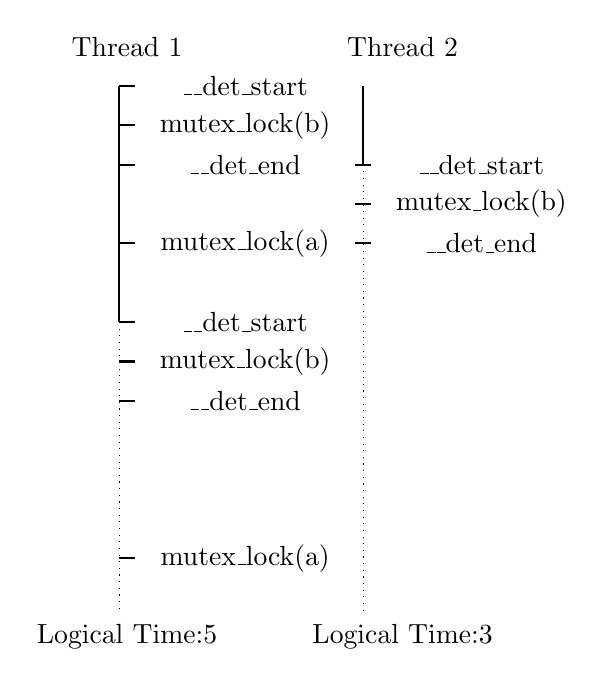
\begin{tikzpicture}
   \draw[thick] (-0.1,4) --  (-0.1,7); 
   \draw[dotted] (-0.1,4) --  (-0.1,0.3);
   
   \node[align=right] at (0,7.5) {Thread 1};
   
   \node[align=right] at (1.5,7) {\_\_det\_start};
   \draw[thick] (-0.1,7) -- (0.1,7);
   \node[align=right] at (1.5,6.5) {mutex\_lock(b)};
   \draw[thick] (-0.1,6.5) -- (0.1,6.5);
   \node[align=right] at (1.5,6) {\_\_det\_end};
   \draw[thick] (-0.1,6) -- (0.1,6);
   \node[align=right] at (1.5,5) {mutex\_lock(a)};
   \draw[thick] (-0.1,5) -- (0.1,5);      
   
   \node[align=right] at (1.5,4) {\_\_det\_start};
   \draw[thick] (-0.1,4) -- (0.1,4);
   \node[align=right] at (1.5,3.5) {mutex\_lock(b)};
   \draw[thick] (-0.1,3.5) -- (0.1,3.5);
   \node[align=right] at (1.5,3) {\_\_det\_end};
   \draw[thick] (-0.1,3) -- (0.1,3);
   \node[align=right] at (1.5,1) {mutex\_lock(a)};
   \draw[thick] (-0.1,1) -- (0.1,1);   
   \node[align=right] at (0,0) {Logical Time:5};
      %show thread 1 holds the lock previously

   \draw[thick] (3,6) --  (3,7); 
   \draw[dotted] (3,6) --  (3,0.3);
   
   \node[align=right] at (3.5,7.5) {Thread 2};
   \node[align=right] at (4.5,6) {\_\_det\_start};
   \draw[thick] (2.9,6) -- (3.1,6);
   \node[align=right] at (4.5,5.5) {mutex\_lock(b)};
   \draw[thick] (2.9,5.5) -- (3.1,5.5);
   \node[align=right] at (4.5,5) {\_\_det\_end}; 
   \draw[thick] (2.9,5) -- (3.1,5);   
   \node[align=right] at (3.5,0) {Logical Time:3};
\end{tikzpicture}
\caption{An example of deadlock}
\label{fig:deadlock}
\end{figure}

\section{Related Work}
Deterministic systems have been studied for a long time. From the implementation perspective view, they can be categorized into 4 different genres: language level, runtime level, OS level and architectural level.

% Use subsections to address each work
% To be fullfilled

Clik++~\cite{leiserson2010cilk++} is an parallel extension to C++ which makes creating parallel program easier. This extension provides a property that can indicate threads to be executed in a serial way, so that the determinism can be ensured. Grace \cite{berger2009grace} is also a C++ extension that adds a fork-join parallel schema to C++, it enforces the determinism of the execution with its underlying language runtime. Both of them are very limited to a specific parallel programming model, and existing applications need to be rewritten to achieve determinism.

Kendo\cite{olszewski2009kendo}, Parrot\cite{cui2013parrot} and Dthreads\cite{liu2011dthreads} provide runtime substitutions for pthread library. By making pthread synchronizations to be deterministic, any race-free pthread-based application can be executed in a deterministic way. They are easy to be applied onto existing applications. However they are limited to pthread only applications. Although Melchior can only make pthread to run deterministically in an automatically way, a developer is always free to use the runtime system calls to hand tune any type of parallel applications to make them deterministic. Among these three, Kendo uses the same deterministic scheduling policy as Melchior. However it relies on hardware counters to keep track of the program's progress in runtime, given the fact that hardware counters could be non-deterministic\cite{weaver2008can}, we doubt the determinism  of Kendo in some cases. DMP\cite{devietti2009dmp} provides an OS layer to make any program running on top of it deterministic, which is applicable for all kinds of parallel programming models. However DMP's overhead is too high due to massive trapping to shared memory accesses. We synchronization provided by the programming model, this could be unnecessary.

In \cite{segulja2012architectural}, an architectural solution is proposed. It's a hardware layer between the CPU core and memory hierarchy, the goal is to track all the memory access and does versioning on the memory operations. By doing deterministic submission to the memory hierarchy, it ensures the determinism of the parallel execution. Although it's a promising solution which is totally transparent to the upper layer, it's not usable out of box in recent years. 
\chapter{Nigoki: Schedule Replication System} \label{chap:schedrep}
In chapter ~\ref{chap:detexec} we described using a deterministic system to ensure the applications on the primary and secondary replica can have the same thread interleaving. The major advantage of the deterministic system is that we can minimize the communication between the replicas. However the downside is that we need to precisely adjust the logical time to maintain decent parallelism for multithreaded applications. We showed various solutions to balance the logical time because we need to keep the execution to be fast and deterministic. If all the burdens come from being deterministic, can we break the determinism once for all but still keep the replicas to be synchronized? The answer is yes.

In this chapter we are going to describe Schedule Replication for replicated applications. In this algorithm, we break the determinism entirely and use messages to synchronize every single synchronization primitives between the primary and replica. For an application that has massive number of synchronization primitives, this approach might introduce overheads from the communication, Figure~\ref{f:tradeoff} shows the relation between two different algorithms. Fortunately, our system is for inter-kernel replication, and Popcorn Linux provides a messaging layer with negatable latency. As a result having massive massages between replicas won't put too much overhead to the replication.

\begin{figure}
\centering
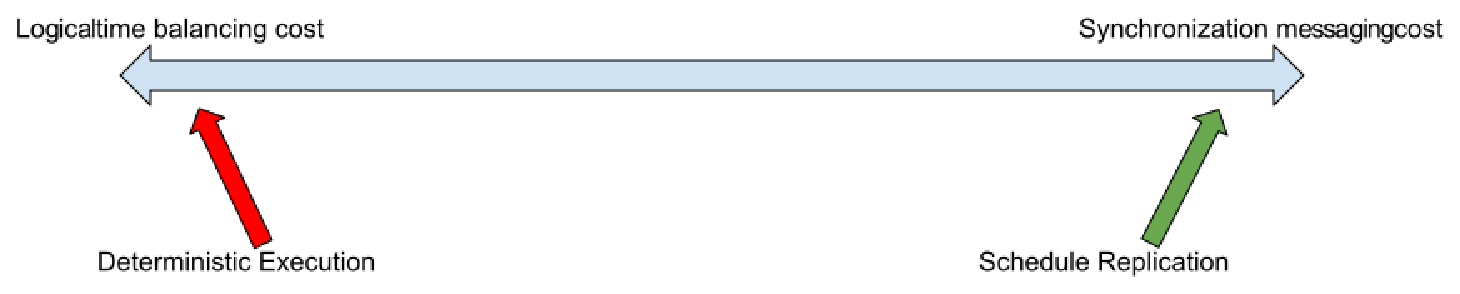
\includegraphics[width=0.8\columnwidth]{figures/tradeoff}
\caption{Trade off between two algorithms}
\label{f:tradeoff}
\end{figure}

\section{Execute-Log-Replay}
Before we get into the detail of this algorithm, let's revisit some important properties that are provided by the deterministic system.

\begin{itemize}
\item Serialization of deterministic areas. (The code region between detstart and detend).
\item Same total order of getting into deterministic areas on primary and secondary.
\end{itemize}

The first property is guaranteed by the fact that the logical time won't change during the execution of a deterministic area, and the second property is guaranteed by increasing the logical time in a same way on both primary and replica. As long as these two properties are guaranteed, the thread interleaving on both primary and secondary are sure to be the same (also for tick bump). In our Schedule Replication mode, we guarantee these two properties with the following approaches:

\begin{itemize}
\item Serialize deterministic areas with a global mutex on both primary and secondary.
\item Log the sequence of getting into deterministic areas on the primary and replay it on the secondary.
\end{itemize}

Here we still use \detstart\ and \detend\ to wrap around a code section that needs to be synchronized with the replica. Figure~\ref{f:schedrep_code} shows a simplified version of \detstart\ and \detend\ in Schedule Replication.

\begin{figure}
\begin{lstlisting}[numbers=left, frame=single, basicstyle=\small, breaklines]{schedrep}
void __det_start()
{
    if (is_secondary(current))
        wait_for_sync(current->seq, 
            ns->seq, current->ft_pid);
    lock(ns->global_mutex);
    current->ft_det_state = FT_DET_ACTIVE;
}
void __det_end()
{
    if (is_primary(current))
        send_sync(current->seq, 
            ns->seq, current->ft_pid);
    current->seq++;
    ns->seq++;
    current->ft_det_state = FT_DET_INACTIVE;
    unlock(ns->global_mutex);
}
\end{lstlisting}
\caption{Simplified implementation of system calls for schedule replication}
\label{f:schedrep_c}
\end{figure}

Figure~\ref{f:schedrep} shows an example of how Schedule Replication works in action.

\begin{figure}
\centering
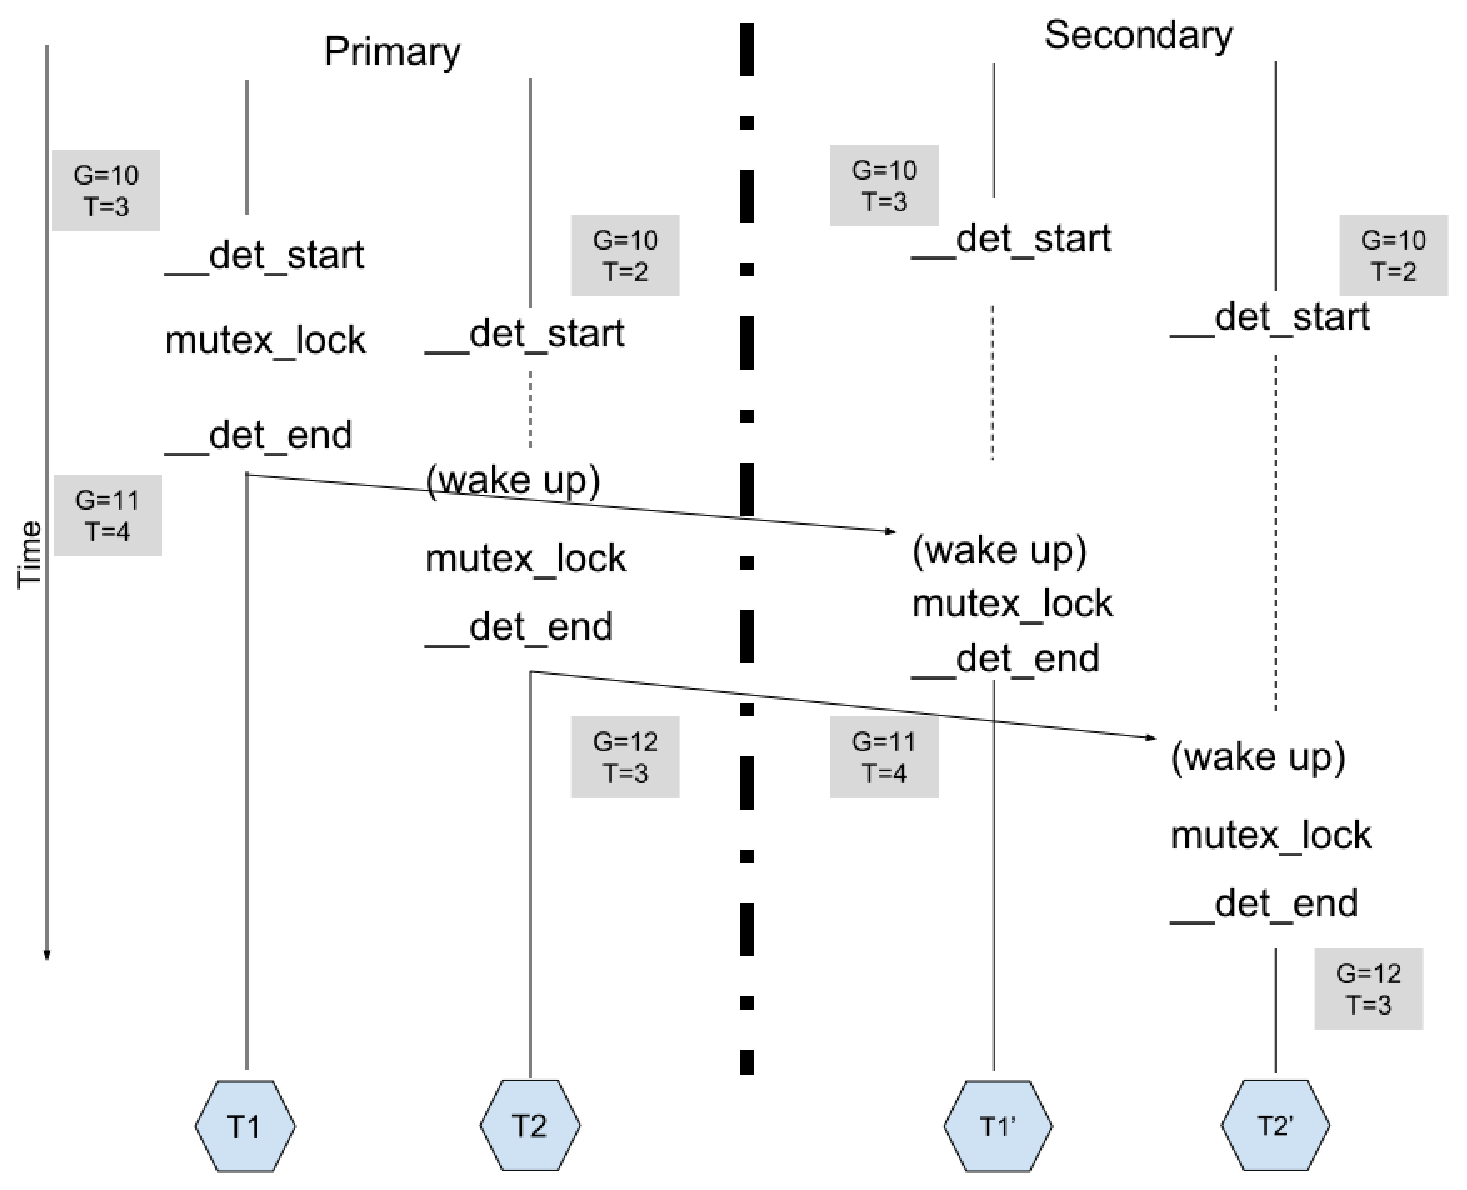
\includegraphics[width=0.9\columnwidth]{figures/sched_rep}
\caption{An example of Schedule Replication}
\label{f:scherep}
\end{figure}

\section{Related Work}

%REX

%ALL about EVE
\chapter{Additional Runtime Support}
With the implementation of the thread synchronization interface, we are able to control the thread interleaving for all the regions surrounded by \_\_det\_start and \_\_det\_end. In this chapter we will discuss the additional runtime support which eliminates some other non-deterministic facts that cannot be simply solved by \_\_det\_start and \_\_det\_end, and some optimizations to the current runtime. This chapter is organized as follows:

\begin{itemize}
  \item Section ~\ref{sec:syscall} shows the non-deterministic facts come from some system calls and our system call synchronization mechanism.
  \item Section ~\ref{sec:library} shows how we instrument pthread primitives with \_det\_start and \_\_det\_end transparently.
  \item Section ~\ref{sec:stdxxx} shows how we create a consistent stdin, stdio and stderr interface for the replicated process.
  \item Section ~\ref{sec:elision} shows an optimization for our system that allows relaxed determinism.
\end{itemize}

\section{System Call Synchronization} \label{sec:syscall}
% put syscall hooks here??
During the execution of an application, for most of the system calls, given the same external input, the application on both primary and secondary can produce the same result, however there are still some system calls that are intrinsically non-deterministic, which will lead to divergence of the execution on all the replicas. As a result we have to synchronize the output of them to ensure the consistent final output of the applications on both sides.

\paragraph{Disabling vDSO}

vDSO(virtual dynamic shared object) is a mechanism that allows a system call to be done in user space, instead of having context switch to the kernel space. This is done by having a shared memory section between the user space and the kernel. When the system call is initiated, the corresponding function in the vDSO library is called instead of trapping into the kernel, then the library will fetch the result from this shared memory area and return. This boosts the performance for some "read only" system calls (like gettimeofday/time). However, in our case, if the system call does not go into the kernel space, we cannot track and synchronize them. Also, in order to synchronize the system call data we have to get into the kernel space anyway to send inter-kernel messages. So vDSO in our context becomes a burden to the implementation. As a result in our system we have to disable vDSO.

In Popcorn Linux, socket read/write/accept/close are already synchronized via the replicated network stack, here we implemented some other system calls that are strongly related to I/O results: 
\begin{itemize}
\item gettimeofday
\item time
\item poll
\item epoll\_wait
\end{itemize}

We did not implement select because it is relatively out-dated, modern network applications hardly use it. In the following subsections we will describe each synchronized system call in detail.

\subsection{gettimeofday/time}

gettimeofday and time are used for getting the current timestamp. Since the primary and secondary can not always have the same execution progress, the timing of calling gettimeofday/time might be different. For those applications that the output is time related, those system calls will cause output divergence. For gettimeofday/time, the primary simply copies the result to the secondary, when secondary executes the corresponding gettimeofday/time, it directly uses the output from the primary and bypasses its original path.

\subsection{poll}

poll is used for waiting on a set of file descriptors for I/O. A programmer can register a set of file descriptors to poll along with the type of events that is related to those file descriptors. poll takes an array of pollfd struct as shown in Figure~\ref{f:pollfd}. When it is called, it waits until one or more registered file descriptors become ready with registered events. When it returns, it fills the array with those file descriptors that are ready and returns the number of ready file descriptors. The user space application iterates the array and reacts to each file descriptor according to the events and revents field.

\begin{figure}
\begin{lstlisting}[numbers=left, frame=single, basicstyle=\small, breaklines]{poll}
int poll(struct pollfd *fds, nfds_t nfds, int timeout);

struct pollfd {
    int   fd;         /* file descriptor */
    short events;     /* requested events */
    short revents;    /* returned events */
};
\end{lstlisting}
\caption{poll prototype and pollfd data structure}
\label{f:pollfd}
\end{figure}

poll notification mechanism relies on the Linux VFS subsystem. However, as described in previous chapter, on the secondary kernel the replicated TCP/IP stack will bypass the original execution path for accept/read/write on sockets, in other words, the VFS subsystem is partially bypassed. As a result, poll will not be woken up properly on the secondary even when the event already arrives, which leads to a different output other than the primary.

The solution is similar to time/gettimeofday, we simply send the output of poll to the secondary. As shown in Figure~\ref{f:pollfd}, the output of poll is the fds array and the return value. Upon receives the information, the secondary uses this as the output of itself and bypasses its original execution path.

\subsection{epoll\_wait}
Similar to poll, epoll\_wait is also used for waiting on a set of file descriptors for I/O. It waits on a set of registered file descriptors and outputs the ready ones to an epoll\_event array. Due to the implementation of our replicated network stack, epoll mechanism has the same problem as poll. Figure~\ref{f:epoll} shows the prototype of epoll\_wait and epoll\_event structure. Compare to the relatively simpe pollfd structure, epoll\_event contains a data field which can be an arbitrary data structure. It is OK to just copy the data field to the other side if it only contains integers. However if this field is a pointer, due to the non-determinism of memory address on both side, simply passing the pointer to the other side may lead to an illegal memory access. As a result, on the secondary, along the output path of epoll\_wait, we need to find the corresponding data structure in its own address space.

On the primary kernel, once the epoll\_wait is ready to return, it will send a message which contains the current epfd, all the ready file descriptors and the value of events field of every file descriptor. Upon the secondary receives the message, it will search the RB tree associated to the given epfd, find the previous registered epoll\_event of the ready file descriptors, and overrides the events field with the information from the primary. At the end, return to the user space with the array of epoll\_event and bypass the original epoll\_wait execution.

\begin{figure}
\begin{lstlisting}[numbers=left, frame=single, basicstyle=\small, breaklines]{epoll}
int epoll_wait(int epfd, struct epoll_event *events,
                      int maxevents, int timeout);

typedef union epoll_data {
    void    *ptr;
    int      fd;
    uint32_t u32;
    uint64_t u64;
} epoll_data_t;

struct epoll_event {
    uint32_t     events;    /* Epoll events */
    epoll_data_t data;      /* User data variable */
};

\end{lstlisting}
\caption{epoll\_wait prototype and epoll\_event data structure}
\label{f:epoll}
\end{figure}

\section{Interposing at Pthread Library} \label{sec:library}
In Chapter~\ref{chap:detexec} and Chapter~\ref{chap:schedrep} we described how to wrap the pthread primitives with \_\_det\_start and \_\_det\_end to ensure the same thread interleaving for the replicated application on the primary and the secondary. Manually instrument the code is tedious, one has to find every single pthread primitive in the code. Moreover, if an application uses an external library that uses pthread, it will be even more troublesome to recompile the needed external library. An intuitive solution is to modify the pthread library and wrap our \_\_det\_start and \_\_det\_end directly in the pthread code. However updating the glibc of a system can be very dangerous and might harm other applications that don't need to be replicated. Fortunately we can use LD\_PRELOAD linker trick to implement a clean solution.

\paragraph{LD\_PRELOAD}
In Linux, the behaviour of the dynamic linker can be altered by setting LD\_PRELOAD environment variable. This can change the runtime linking process and make the linker to search for symbols in the path defined in LD\_PRELOAD. With this trick we are able to alter the behaviour of glibc without actually changing it. We implemented our LD\_PRELOAD library with instrumented pthread functions in it, and the namespace launching script will automatically set LD\_PRELOAD environment variable to be the path of our library, so that only the application running in the namespace will be affected by our LD\_PRELOAD library. In the upcoming sections we will describe how we wrap pthread functions in our LD\_PRELOAD library.

\subsection{Interposing at Lock Functions}

Figure~\ref{f:orverridelocks} shows the implementation of pthread\_mutex\_lock in our LD\_PRELOAD library. Line 9 loads the real pthread\_mutex\_lock function from the real pthread library, in Line 12 we simply call this function with \_\_det\_start and \_\_det\_end wrapped around. In our LD\_PRELOAD library, we wrapped all the pthread lock functions include pthread\_mutex\_lock, pthread\_mutex\_trylock, pthread\_rwlock\_rdlock, pthread\_rwlock\_tryrdlock, pthread\_rwlock\_wrlock, pthread\_rwlock\_trywrlock. There we need no special treatment for unlock primitives, as long as the calling sequence of lock operations are determined, the return timing for the lock operations will follow the same sequence ~\cite{merrifieldincreasing}.

\begin{figure}
\begin{lstlisting}[numbers=left, frame=single, basicstyle=\small, breaklines]{locks}
int pthread_mutex_lock(pthread_mutex_t *mutex)
{
    int ret;
    static int (*pthread_mutex_lock_real)(pthread_mutex_t *mutex) = NULL;    
    if (!handle) {
        handle = dlopen(PTHREAD_PATH, RTLD_LAZY);
    }
    if (!pthread_mutex_lock_real)
        pthread_mutex_lock_real = dlsym(handle, "pthread_mutex_lock");

    syscall(__NR_det_start);
    ret = pthread_mutex_lock_real(mutex);
    syscall(__NR_det_end);

    return ret;
}
\end{lstlisting}
\caption{pthread\_mutex\_lock in the LD\_PRELOAD library}
\label{f:orverridelocks}
\end{figure}

\subsection{Interposing at Condition Variable Functions}

Condition Variables are much more complicated than mutex locks. In the glibc implementation, it involves multiple internal lock and unlock operations. As a result simply wrapping pthread\_cond\_wait with \_\_det\_start and \_\_det\_end will not work, because of multiple non-deterministic execution points are inside the implementation. Figure~\ref{f:cond_wait} shows the brief flow of the pthread\_cond\_wait in glibc implementation, yellow blocks are the lock acquisitions. cond\textrightarrow lock is a lock inside the condition variable  data structure, it is used to provide mutual exclusion for the futex value for the condition variable. futex\_wait will wait until cond\textrightarrow futex differs from futex\_val. When it wakes up, it will check again if this condition variable is contended, if so, go back to futex\_wait again. If not, re-acquire the mutex lock and return. Every single lock acquisition here is a non-deterministic point, which leads to passing different values to futex\_wait on primary and replica, which in turn leads to diverged wakeup timing of pthread\_cond\_wait.

In our LD\_PRELOAD library, we re-implemented pthread\_cond\_wait following the existing glibc's implementation, and wrapped every lock acquisition with \_\_det\_start and \_\_det\_end, we also did the same wrapping for pthread\_cond\_signal. With this, we are able to make sure that the pthread\_cond\_wait can return at the same timing with the same condition variable on both primary and secondary.

%For pthread\_cond\_timed\_wait, we did the same re-implementation for it. However the timeout part is a little bit tricky. %how the fuck can pthread\_cond\_timed\_wait works accidently?

\begin{figure}
\centering
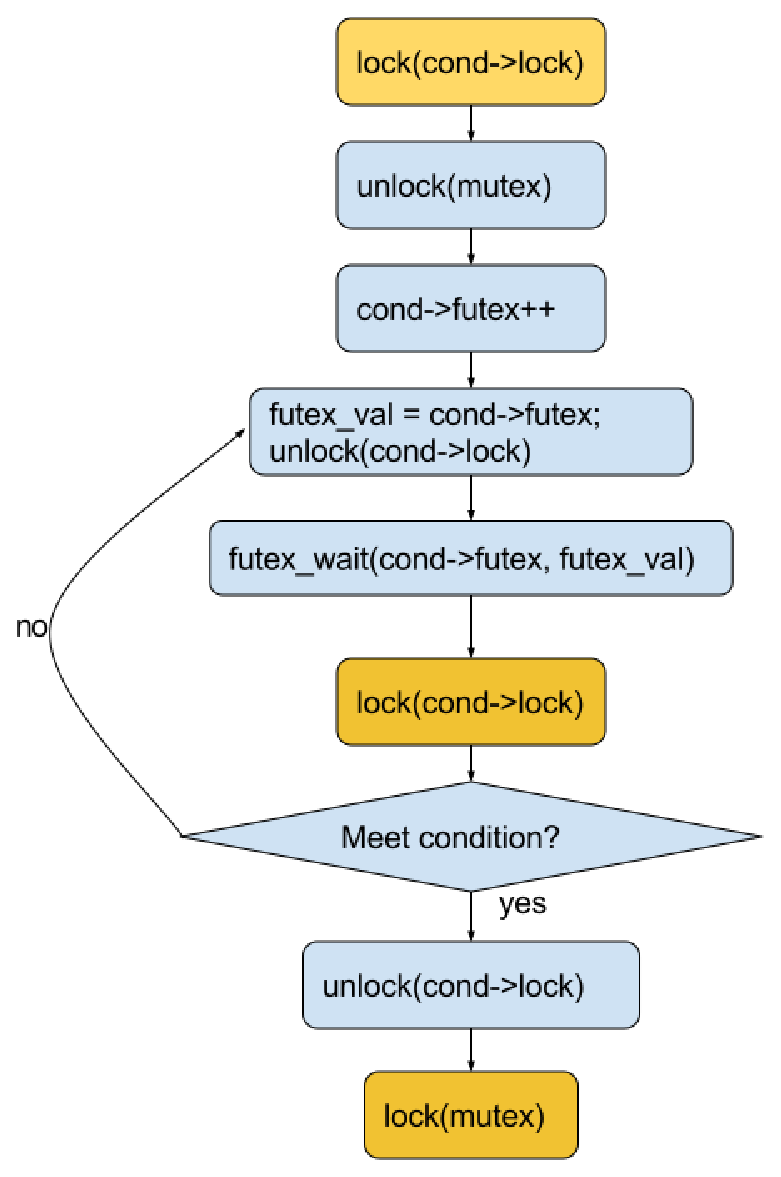
\includegraphics[width=0.4\columnwidth]{figures/cond_wait}
\caption{glibc pthread\_cond\_wait internal work flow}
\label{f:cond_wait}
\end{figure}

\section{stdin, stdio and stderr} \label{sec:stdxxx}

In the booting process of Linux, init is the very first userspace process and it creates the file descriptors for stdin, stdio and stderr. All upcoming processes inherit those three file descriptors from init. This gives all the processes the ability to interact with a terminal device, also gives the fact that 0, 1 and 2 are the "reserved" file descriptor numbers in a process, any newly created file descriptor starts from 3. However, as we described previously, Popcorn Linux generates a replicated process on the secondary from the kernel space, pretty much like how init is created. As a result the replicated process doesn't inherit the stdin, stdio and stderr and newly created file descriptor starts from 0. This creates divergence on applications which take file descriptor numbers as some sort of input. An example is poll and epoll\_wait, since we copy the ready file descriptors on the primary to the secondary, the divergence on file descriptor numbers will lead to unexpected results for upcoming I/O operations after poll or epoll\_wait. The solution is very straightforward, upon the creation of the replicated process on the secondary kernel, we look for an available pts device, and  use it as the terminal for stdin, stdio and stderr of the replicated process. In this way we are able to have consistent file descriptor numbers on primary and replica, and also be able to see the replicated process's console output.

\section{Synchronization Elision} \label{sec:elision}
In some applications, not all the lock acquisition must be synchronized. For example, the lock primitives in a memory allocator don't affect the final output at all, as a result we can relax the determinism for those locks. In both synchronization strategies, we multiplexes \dettick\ with tick number 0 as the hint for relaxing the determinism of the next \detstart\. When that \detstart\ is called, the system call does nothing and simply returns. In this way we are able to boost the performance of some applications with manual instrumentation.
\chapter{Evaluation}

In this chapter we will show some experiment results of our system. We will use various applications which will cover all the aspects of our implementation includes thread interleaving synchronization, application instrumentation and system call synchronization. With all the evaluation, we will answer the following questions:

\begin{itemize}
  \item Correctness: Given the same input, can the primary and secondary consistently generate the same output?
  \item Performance: Compare to non-replicated execution, how much overhead is introduced by our system?
  \item Breakdown: Where does the overhead come from?
\end{itemize}
% Evaluation factors:
% 1. Lock count & pcnmsg count for schedule part
% 2. Breakdown
% 3. Absolute time

\paragraph{Evaluation Setup} All experiments were run on a server machine with 4 AMD Opteron 6376 Processors (16 cores each, 2.3Ghz), which is 64 cores in total. The total RAM is 128GB. Our Popcorn Linux kernel was installed on Ubuntu 12.04 LTS. We partitioned the hardware resources into half, one for the primary and one for the secondary. Each of them has the full control of their own 32 cores and 64GB RAM. The machine comes with a 1Gbps high speed connection. For benchmarking server applications, we used a machine in the same rack, connected to the same switch, to act as the benchmark client.

\section{Racey}
We used a variant of racey~\cite{hillstress} to evaluate the correctness of our system. racey benchmark is a set of concurrent programs which read and write some shared data concurrently with various concurrent models. With a non-deterministic system, all the benchmark will create a different result during each different run. We use racey to validate if we can have the same thread interleaving on primary and secondary, which should lead the same output on both primary and secondary.

\paragraph{racey-guarded} racey-guarded has a global array, it uses pthread to create multiple threads and modify the global array concurrently. The access to the global array is protected by pthread\_mutex\_lock. We tested this one without any modification to the application. With both synchronization algorithms, we are able to create consistent results on the primary and secondary for over 100 consecutive runs.

\paragraph{racey-forkmmap} racey-forkmmap utilizes mmap to create a shared memory area, and uses fork to create multiple processes to read and modify the shared memory area. We manually added \_\_det\_start and \_\_det\_end around each access to the shared memory area. With both synchronization algorithms, we are able to create consistent results on the primary and secondary for over 100 consecutive runs.

\paragraph{racey-tcp} Based on the idea of racey, we developed racey-tcp to stress the determinism for I/O related tasks. racey-tcp uses pthread to create multiple threads. One thread listens to the socket, whenever a new connection arrives, it puts the connection into a queue, other threads retrieve the connection from the queue, read the data on that connection and write the data into a file. For this benchmark, we wrapped the write system call for writing to the file with \_\_det\_start and \_\_det\_end. With both synchronization algorithms, we are able to create consistent output file on the primary and secondary for over 2000 requests.

\section{PBZip2}
% 1. threading model
% 2. A table of lock and cond var count
% 3. A table of instrumented dettick count
PBZip2 is the parallel version of bzip2. The concurrent model of this application is a typical producer-consumer model

% The concurrent model is shown in Figure~\ref{f:pbzip_model}. The FileReader thread reads the content of the file, break the input data into data chunks and put all the chunks into a queue. Worker threads get the data chunks from the queue 


%\begin{figure}
%\centering
%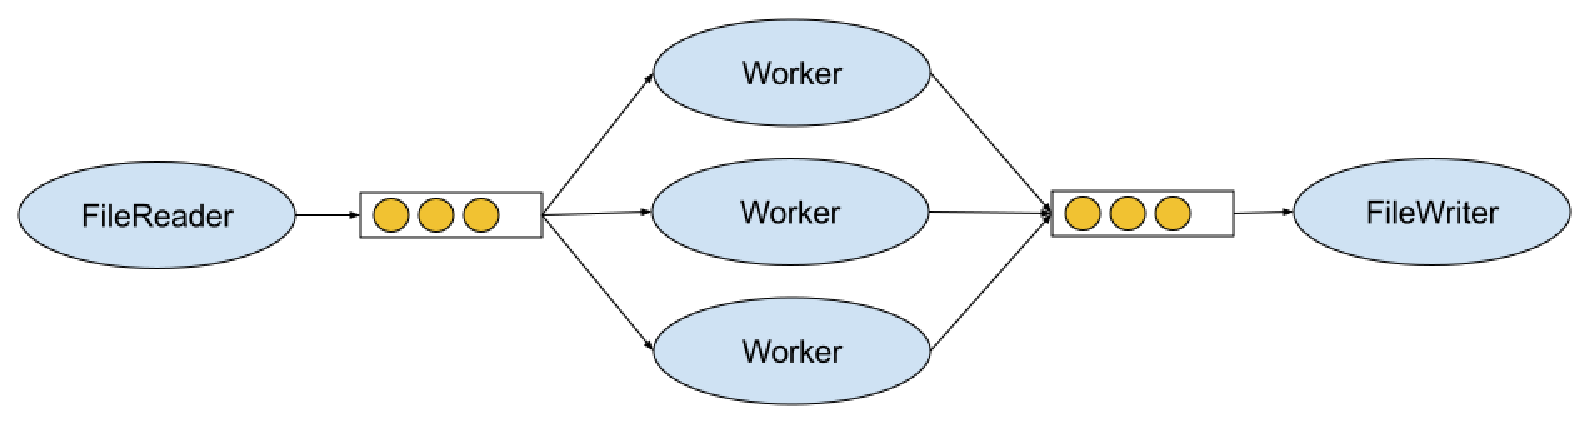
\includegraphics[width=0.8\columnwidth]{figures/pbzip2_model}
%\caption{pbzip2 concurrent model}
%\label{f:pbzip_model}
%\end{figure}


For PBZip2, the time consuming part is the place where it calls the libz2 compression/decompression functions. In this benchmark, we utilized the execution time profiling instrumentation to gain a decent performance in the deterministic execution, while for schedule replication nothing is modified.

Table~\ref{t:pbzip2_syscall} shows the system calls that are used by pbzip2, we only show the system calls that are tracked and synchronized by our system. In pbzip2,  gettimeofday is only used for showing the time spent on the whole process, so it is not critical to the output of the application. But since we synchronized it, both the primary and secondary showed the same finishing time all the time.

\begin{table}
 \caption{Tracked system calls used by pbzip2}
\begin{center}
 \begin{tabular}{c | c}
 System Call & Use in the Application\\ \hline
 gettimeofday & Calculate execution time
 \end{tabular}
\end{center}
\label{t:pbzip2_syscall}
\end{table}

\section{Mongoose Webserver}
% 1. threading model
% 2. A table of lock and cond var count

Mongoose is a compact multithreaded webserver.

Table~\ref{t:mongoose_syscall} shows the system calls that are used by mongoose. In mongoose, both system calls are critical to the final output.

\begin{table}
\caption{Tracked system calls used by mongoose}
\begin{center}
 \begin{tabular}{c | c}
System Call & Use in the Application\\ \hline
 time & Generate HTTP header  \\ \hline
 poll & Wait for accept, read and write
 \end{tabular}
\end{center}
\label{t:mongoose_syscall}
\end{table}

\section{Nginx Webserver}
Nginx is a sophisticated webserver with multiple threading modes.

\begin{table}
\caption{Tracked system calls used by nginx}
\begin{center}
 \begin{tabular}{c | c | c}
System Call & Use in the Application\\ \hline
 time & Generate HTTP header\\ \hline
 poll & Wait for accept, read and write
 \end{tabular}
\end{center}
\label{t:nginx_syscall}
\end{table}


\section{Redis Database Server}
Redis is an in-memory database server. It uses a single thread to process requests, but it dynamically creates new threads to write the in-memory data to the disk. This benchmark is perfect for stressing the flexibility of dealing with dynamically spawned threads.

\subsection{Overhead Profiling}
\subsection{Results}

\chapter{Conclusion}

In this thesis we have explored a novel approach for doing replication: intra-machine replication with a multi-kernel OS. We have shown the challenges of replicating non-deterministic concurrent applications, and implemented two different replication modes to tame the non-deterministic thread-interleaving for concurrent applications. Also with a set of runtime support, we are able to replicate existing applications with minimal modification. With our benchmarks, we have also shown that both replication modes are able to achieve low overhead for different types of  applications.

\section{Contributions}
This thesis presents the following contributions:

\begin{itemize}
\item \textbf{We implemented two different replication modes to synchronize the thread-interleavings and output for replicated concurrent applications.} Both of them achieved the same goal in two different directions: Deterministic Execution uses a deterministic algorithm to decide the order of execution on both primary and secondary; while Schedule Replication enforces the secondary replica to follow the non-deterministic execution order that happened previously on the primary kernel.

\item \textbf{For Deterministic Execution, we developed a compiler framework to automatically instrument the application code to increase parallelism.} The compiler framework can profile the application and generate approximate values to increasing the logical time at the end of time consuming basic blocks. By balancing the logical time with instrumented values, the application can achieve decent overhead and scalability in Deterministic Execution.

\item \textbf{Based on the common programming interface for both replication modes, we implemented a set of runtime support to eliminate the non-determinism in pthread library.} By wrapping a code section with \detstart\ and \detend\ system calls, the execution order of wrapped sections can be the same on both primary and secondary kernel. We implemented an instrumented pthread library that can be dynamically linked with LD\_PRELOAD technique, which can minimize the effort of modifying the applications code. \textbf{For our evaluation, we did no modification to pbzip2, added 1 line to mongoose and added around 60 lines to nginx}.

\item \textbf{We evaluated both replication modes with different concurrent applications. Our system showed decent overhead on both replication modes.} For a computational, non-network application we had \textbf{14.27\% to 63.39\%} slowdown for Deterministic Execution and maximum \textbf{0.89\% to 36.3\%} slowdown for Schedule Replication. For two web servers we had maximum \textbf{1.6\% to 25.22\%} slowdown for Deterministic Execution and maximum \textbf{0.23\% to 1.96\%} slowdown for Schedule Replication.

\end{itemize}
\section{Future Work}
\subsection{Precise Tick Bump for Deterministic Execution}
The major overhead in Deterministic Execution is the imbalanced logical time. The more precise the logical time incremental is the less waiting time we spend on \detstart\ . In chapter ~\ref{chap:detexec} we described our solution with a profiling approach, but from the evaluation we see this is still not precise enough to have the best performance. While performance counters are not deterministic enough to do the job~\cite{weaver2008can}, Intel PT~\cite{intelpt} seems to be a promising approach to track the progress of the execution. PT is able to precisely track the actual behaviour of the execution (e.g. branch decisions) not just a counter of software events, as a result for the same executable, same input and same thread-interleaving, PT should always generate the same execution trace and be deterministic. With this dynamic tracing technique, we might be able to provide precise online tick bumping without having to instrument the code.
\subsection{Pre-Lock Synchronization}
From the benchmark results, we occurred more overhead when the type of locks increases. This is because with serializing all the lock acquisitions, we are breaking the parallelism of accessing of different locks. If we only synchronize the access order of each particular lock while relaxing the total order of all the other locks, we might be able to achieve higher parallelism.

We could give an unique ID to \detstart\ as an additional parameter to identify different deterministic sections. However, the reason we couldn't implement this is that there is no perfect solution to generate this ID. A naive solution is to manually instrument the code with \detstart\ and \detend\, and manually assign an ID to each deterministic section. This requires massive changes to existing code. Moreover, some applications require external libraries that includes lock primitives which makes this even harder.

For pthread primitives, given the fact that most of them have futex involved, we could use the futex address~\cite{drepper2005futexes}~\cite{franke2002fuss} as the unique IDs for each deterministic section. However during our test we found the primary and secondary replica cannot always have the same address for the same lock. This is expected because they are on separate Linux kernels and have different address spaces. Some deterministic systems address the problem of non-deterministic memory address allocation and mitigated the problem with modified memory allocator ~\cite{bergan2010deterministic}~\cite{liu2011dthreads}, in the future if we are able to synchronize the address space on the replicas, we might be able to directly use futex addresses as IDs for deterministic sections and achieve transparent pre-lock synchronization. 

\subsection{Arbitrary Number Replicas}
%cite consensus here, mention paxos made transparent, rex
%Address how increasing replicas can impact speed for schedule replication
Current implementation only supports one primary replica and one secondary replica. However Popcorn Linux supports booting arbitrary number of kernels as long as the hardware has enough resources. It would be interesting to explore the possibility of having more than one secondary replica. The major challenge is to decide the communication model for multiple replicas.

One solution is to do "Chain-Messaging". In this model we chain all the replicas one by one, the primary sends replication messages to the 2nd replica, and 2nd replica sends messages to 3rd replica and so on. Since point to point messaging is sure strictly FIFO on Popcorn Linux, this approach makes sure that all the replicas will see the same sequence of replication messages. Another advantage is that this can minimize the latency for the primary replica since it only communicates with one kernel. However in this approach the performance of the nth replica will be held back by all previous n-1th replicas, it cannot proceed until all its previous replicas have committed their operations.

We can also do broadcasting from the primary replica. Since we don't have the guarantee that message broadcasting in Popcorn Linux can behave in strictly FIFO, we might need to introduce consensus protocol such as Paxos ~\cite{lamport2001paxos} to make sure that all the replicas see the requests in the same order.

Another challenge is that when multiple replicas involved, who is going to be the primary when the previous primary fails. This can also be solved by utilizing the leader selection mechanism of Paxos ~\cite{lamport2001paxos}.

\subsection{Hybrid Replication}
%same, cite consensus here, mention paxos made transparent, rex

It is also interesting to extend this work to inter-machine and intra-machine hybrid replica. We can use intra-machine replica to deal with processor and memory faults with fast recovery, and inter-machine backup to deal with critical power failure with slower recovery. This will also have the same consensus problems as we mentioned in the previous section.

In our intra-machine implementation, we benefit a lot from our low latency messaging layer, the average time for sending a message is below 5 microseconds. However in a inter-machine setup, we might see different result than what we showed in our evaluation. The higher cost of inter-machine communication might cause greater slow down in Schedule Replication. While for Deterministic Execution which usually needs less messages, it might perform better than Schedule Replication in this case.

\bibliographystyle{unsrt}
\bibliography{bibliography}

\end{document}

